\section{Rückblick}

\author{Erivn Mazlagi\'c}

\subsection{Projektmanagement}
\begin{frame}
	\frametitle{Projektmanagement\hfill{}\footnotesize \group}
	\framesubtitle{Kollaboratives Projektmanagement}
	\begin{block}{Merkmale (Quelle: Wikipedia)}
		\begin{itemize}
			\item Projektmanagement ist Aufgabe aller Teilnehmer
			\item Dezentraler Regelkreis $\rightarrow$ Aufteilung des PM in Fachbereiche
			\item Vernetzung \& Synchronisation $\rightarrow$ gemeinsame Planungsbasis
			\item Zentrale Datenbasis $\rightarrow$ erlaubt getrenntes Arbeiten
			\item Kommunikaiton \& Kollaboration $\rightarrow$ Transparenz \& Kontrolle
		\end{itemize}
	\end{block}
\end{frame}

\begin{frame}
	\frametitle{Projektmanagement \hfill \footnotesize \group}
	\framesubtitle{Kollaboratives Projektmanagement}
	\begin{columns}
		\begin{column}{0.7\textwidth}
			\begin{block}{Umsetzung (Quelle: Wikipedia)}
				\begin{itemize}
					\item Proaktive \& toolsgestützte Kollaboration
					\item Zentrale Datenbasis
					\item Klar zugeteilte Verantwortlichkeiten
					\item Top-Down-Vorgabe von Meilensteinen
					\item Intuitive Vernetzung für Abstimmungen
				\end{itemize}
			\end{block}
		\end{column}
		\pause
		\begin{column}{0.3\textwidth}
			\begin{exampleblock}{Team 39}
				\begin{itemize}
					\item git
					\item GitHub
					\item Issues
					\item Milestones
					\item Comments
				\end{itemize}
			\end{exampleblock}
		\end{column}
	\end{columns}
\end{frame}

\subsection{Projektverlauf}
\begin{frame}
	\frametitle{Projektverlauf\hfill{}\footnotesize \group}
	\framesubtitle{Eine graphische Analyse}
	\begin{figure}
		\centering
		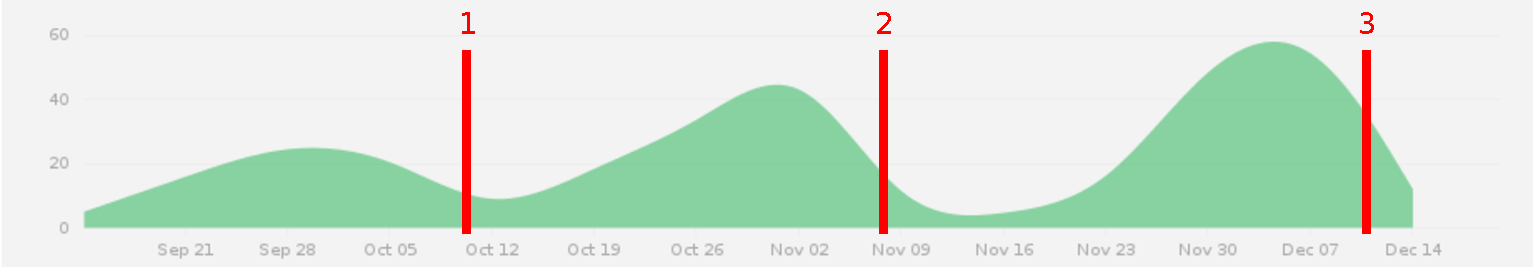
\includegraphics[width=1\textwidth]{../../fig/pm/gh-contributions-ov_marked.pdf}

		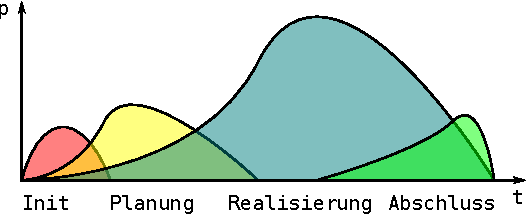
\includegraphics[width=0.5\textwidth]{../../fig/pm/pm-phasen.pdf}
		\caption{Contributions vs. idealem Projektzyklus}
	\end{figure}
\end{frame}

\begin{frame}
	\frametitle{Projektverlauf\hfill{}\footnotesize \group}
	\framesubtitle{Visualisierung mit gource}
	\begin{columns}
		\begin{column}{0.5\textwidth}
			\begin{block}{Gerenderte Animation von github.com/accefa/doku}
				\movie[width=4cm,height=4cm, externalviewer]{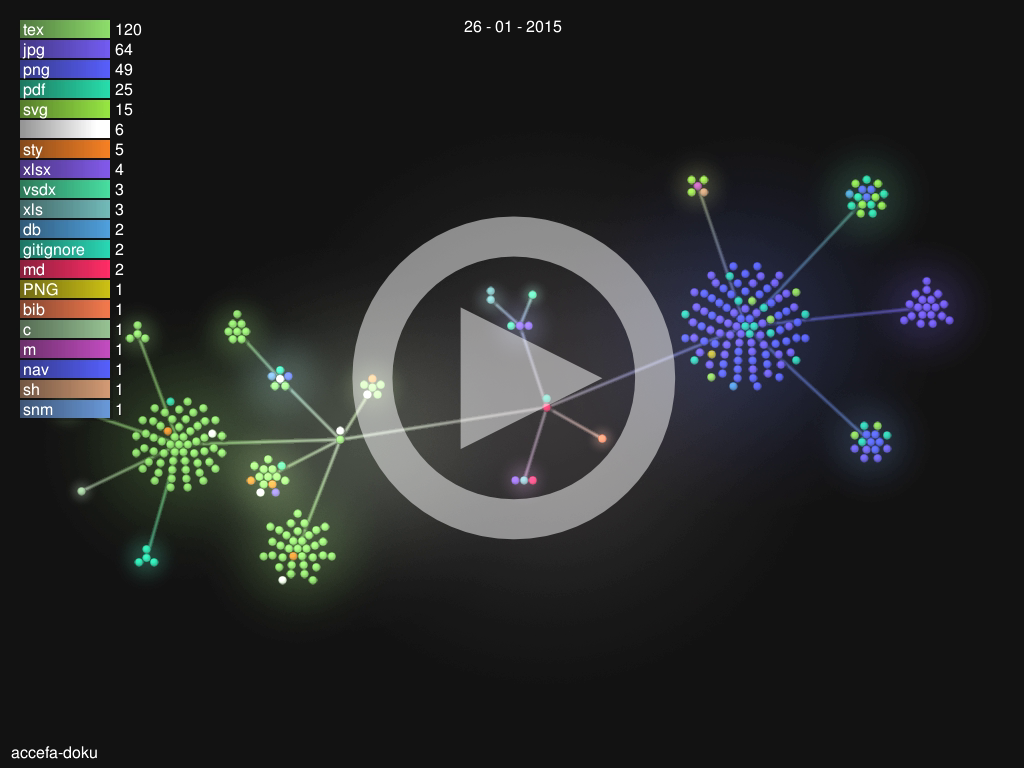
\includegraphics[width=1\textwidth]{../../fig/gource_play.png}}{gource-dark.mp4}
				\\ gource-dark.mp4 \hfill{} 1:24 min
			\end{block}
		\end{column}
		\begin{column}{0.5\textwidth}
			\begin{exampleblock}{gource Parameter}
				\lstinputlisting{gource-commands.txt}
			\end{exampleblock}
		\end{column}
	\end{columns}
\end{frame}
